\scanpage{340}
% R340.01 | text | top, lines 1--12 | Ce calcul suggère fortement
This calculation strongly suggests that the relations \deleted{\unsure{pa|by}} (64) already imply (68)\ldots{} it is \unsure{even} very nearly a proof\ldots{} If we admit this point, it only remains to verify that the preceding conditions \inserted{(64)} (i.e. essentially already (51) to (56) except (55)) also imply (55), i.e. the independence of the $\varepsilon_0,\varepsilon_1$ in every fiber, i.e. that $N_0,N_1$ are non-homothetic in \unsure{every} fiber. Now (67)
% R340.02 | display | upper middle, line 13 | N_1=tilde sigma(N_0)
\[
(*)\qquad N_1=\widetilde\sigma(N_0),\ \unsure{\deleted{\text{and}}}\ \inserted{=\widetilde\rho(\unsure{N_1|N_0})}\ \deleted{N_0=\unsure{\widetilde\sigma(N_1)}}\,\unsure{:}
\]
% R340.03 | text | middle, line 14 | Si on avait sur une fibre
If we had on a fiber
% R340.04 | display | middle, line 15 | N_1=lambda N_0
\[
\unsure{(\deleted{74})}\qquad N_1=\lambda N_0
\]
% R340.05 | text | middle, lines 16--18 | on en conclurait
we would conclude from this, by \unsure{applying} \deleted{$\widetilde\sigma$ and} using $\widetilde\sigma^2=1$, \inserted{and $\widetilde\rho^3=1$,} \inserted{the relations} \deleted{$\widetilde\sigma(N_1)=N_0$, $\widetilde\sigma(N_0)=N_1$}
% R340.06 | display | lower middle, lines 19--20 | N_0=lambda N_1
\[
\deleted{\unsure{(**)}\qquad
\left\{\begin{aligned}
N_0&=\lambda N_1\unsure{\deleted{=\lambda^2}},\quad
\text{thus }\deleted{\lambda^2=1}\ N_0=\lambda^2N_0\quad\text{whence}\\
\lambda^2&=1.
\end{aligned}\right.}
\]
% R340.07 | text | lower middle, line 21 | Mais un calcul immédiat
\deleted{But an immediate calculation also gives}
% R340.08 | display | lower middle, line 22 | N_0=rho^{-1}N
\[
\deleted{(**)\qquad N_0=\rho^{-1}N,\quad N_1\unsure{-}}
\]
% R340.09 | display | lower, line 23 | lambda^2=1,lambda^3=1
\[
\lambda^2=1,\quad\lambda^3=1\qquad\text{whence }\lambda=1
\]
% R340.10 | text | lower, lines 24--28 | i.e. N_0=N_1
i.e. $N_0=N_1$ i.e. $N_0$ commutes with $\sigma,\rho$ thus also $N=-\sigma N_0$ \inserted{$=\rho^{-1}N_0$} commutes with $\sigma,\rho$, and since $N=\sigma+\rho$, $\sigma$ and $\rho$ commute. But then
% R340.11 | text | bottom left | 339
\mspage{339}

\scanpage{341}
% R341.01 | text | top centre | 471
\mspage{471}
% R341.02 | display | top, lines 1--2 | (sigma+rho)^2
\[
(\sigma+\rho)^2=\underbrace{\sigma^2}_{-1}+\underbrace{\rho^2}_{\rho-1}+2\sigma\rho=\rho-2+2\sigma\rho=
\]
% R341.03 | text | upper, line 3 | donc la relation
thus the relation $(\sigma+\rho)^2=\sigma+\rho$ is written
% R341.04 | display | upper, lines 4--5 | rho-2+2 sigma rho
\[
\deleted{\rho}-2+2\sigma\rho=\sigma+\deleted{\rho}\qquad\text{i.e.}
\]
\[
\deleted{\unsure{(**)}}\qquad
2\sigma\rho=\sigma+2\quad\text{that is}\quad
\underbrace{2\sigma^2\rho}_{-2\rho}=\underbrace{\sigma^2}_{-1}+2\sigma
\quad\text{i.e.}\quad 2(\sigma+\rho)=1
\]
% R341.05 | text | upper middle, lines 6--14 | Prenant les traces
\deleted{Taking the traces of both sides, and using $\operatorname{Tr}\sigma\rho=2$ (74), $\operatorname{Tr}\sigma=0$, $\operatorname{Tr}1=2$, we find $4=4$, no contradiction but taking the determinants \inserted{of both sides of \unsure{(**)},} we find (\deleted{\unsure{det}} admitting that $\det\sigma=\det\rho=1$, which is a consequence of (64) provided only that we require in addition that $\sigma,\rho$ be regular i.e. be scalars on no fiber) we find}
% R341.06 | margin note | left of lines 12--14 | double vertical stroke
\margin{$\Vert$}
% R341.07 | display | middle, line 15 | 2^2=2^2+2 Tr sigma
\[
\deleted{(***)\qquad 2^2=2^2+2\underbrace{\operatorname{Tr}\sigma}_{0}+\underbrace{(\det\sigma)^{\unsure{2}}}_{1}\quad\text{i.e.}\quad 1=0}
\]
% R341.08 | text | middle, lines 16--17 | ce qui est absurde
\deleted{which is absurd. whence, taking}

\deleted{I \unsure{it}} i.e.
% R341.09 | display | lower middle, line 18 | 2N=1
\[
(**)\qquad 2N=1,
\]
% R341.10 | text | lower middle, line 19 | d'où, en prenant
whence, taking the determinants
% R341.11 | display | lower middle, line 20 | 4 det N=1
\[
4\underbrace{\det N}_{0}=1\qquad\text{i.e.}\quad 0=1,\quad\text{\uline{absurd}.}
\]
% R341.12 | text | lower, lines 21--25 | Remarque Je ne serais pas étonné
\deleted{I will not be}

\uline{Remark} I would not be surprised if we also had conditions equivalent to (51) to (56) in the form
% R341.13 | display | bottom, line 26 | (75) sigma^2+1
\[
(75)\qquad \sigma^2+1=\rho^{\unsure{3|2}}\unsure{-|+}\rho+1=0,\quad
\varepsilon_0\mathrel{\overset{\mathrm{dfn}}{=}}-\sigma^{-1}\rho\ \text{is regular unipotent}
\]
% R341.14 | text | bottom left | 340
\mspage{340}

\scanpage{342}
% R342.01 | text | top, lines 1--4 | en exigeant de plus
requiring in addition, if need be, that $\sigma,\rho$ also be regular i.e. be scalars on no fiber. One would have to convince oneself that this implies that
% R342.02 | display | upper, line 5 | N=dfn rho+sigma
\[
N\mathrel{\overset{\mathrm{dfn}}{=}}\rho+\sigma
\]
% R342.03 | text | upper, line 6 | satisfait bien la relation
does satisfy the idempotence relation
% R342.04 | display | upper, line 7 | N^2-N=0
\[
(75)\qquad N^2-N=0
\]
% R342.05 | text | upper middle, line 8 | ce qui équivaut
(which is equivalent, if $N$ regular, to
% R342.06 | display | upper middle, line 9 | Tr N=1,det N=0
\[
(77)\qquad \operatorname{Tr}N=1,\quad\det N=0\qquad (?)
\]
% R342.07 | text | middle, lines 10--13 | Mais N est régulier
But $N$ is regular, for if on a fiber \unsure{it were} a scalar we would have that (restricting to this fiber) $\rho$ and $\sigma$ commute, we would have
% R342.08 | display | middle, lines 14--15 | -sigma^{-1}rho=sigma rho
\[
\begin{aligned}
-\sigma^{-1}\rho&=\sigma\rho=\varepsilon_0=1+N_0\\
-\inserted{\unsure{''}}\rho\sigma^{-1}&=\rho\sigma=\varepsilon_1=1+N_1,
\end{aligned}
\]
% R342.09 | deletion | middle, beneath second epsilon identity | Prenant
\deleted{\unsure{Taking} $\unsure{\varepsilon_0=\det\rho}$}

\deleted{with}
% R342.10 | display | middle-lower, lines 16--18 | (1-sigma rho)^2=0
\[
(1-\sigma\rho)^2=0\quad\text{i.e.}\quad
1-2\sigma\rho+\underbrace{\sigma^2}_{-1}\underbrace{\rho^2}_{\rho-1}=0\quad\text{i.e.}
\]
\[
1-2\sigma\rho+1-\rho=0\quad\text{i.e.}\quad 2=\rho+2\sigma\rho
\]
% R342.11 | text | lower, line 19 | soit, en multipliant
that is, multiplying by $\sigma$
% R342.12 | display | lower, line 20 | 2 sigma=rho sigma+2 sigma^2 rho
\[
2\sigma\unsure{=}\rho\sigma+2\underbrace{\sigma^2}_{-1}\rho
\quad\text{i.e.}\quad 2\underbrace{(\sigma+\rho)}_{N}=\rho\sigma
\]
% R342.13 | text | lower, lines 21--23 | Mais par hyp.
But by hypothesis we have $N=\lambda.1$, $\lambda$ a scalar, whence $\rho\sigma=2\lambda$, and taking the determinants
% R342.14 | display | lower, line 24 | det(rho sigma)=4 lambda^2
\[
\det\underbrace{(\rho\sigma)}_{1}=4\lambda^2
\]
% R342.15 | text | bottom, line 25 | i.e. 2 inv.
i.e. $\deleted{\unsure{4}}\ 2$ invertible and $\lambda=\dfrac{\varepsilon}{2}$, with $\varepsilon^2=1$,
% R342.16 | display | bottom, lines 26--27 | rho sigma=epsilon
\[
\begin{aligned}
\text{i.e.}\qquad&\rho\sigma=\varepsilon\qquad\varepsilon^2=1,\\
&\rho^2\underbrace{\sigma^2}_{-1}=1\qquad\underbrace{\rho^2}_{\rho-1}=-1,\quad\text{i.e.}\quad\rho=0,\quad\text{\uline{absurd}}
\end{aligned}
\]
% R342.17 | text | bottom left | 341
\mspage{341}

\scanpage{343}
% R343.01 | text | top centre | 472
\mspage{472}
% R343.02 | deletion | top, line 1 | Mais Tr N=0
\deleted{But $\operatorname{Tr}N=0$ \unsure{by}}
% R343.03 | text | upper, lines 2--4 | Donc N est régulier
Thus $N$ is regular, it remains to prove (77).

But $\operatorname{Tr}N=\underbrace{\operatorname{Tr}\sigma}_{0}+\underbrace{\operatorname{Tr}\rho}_{1}=1$, OK, remains to prove $\det(\rho+\sigma)=0$ but
% R343.04 | display | upper middle, line 5 | det(rho+sigma)
\margin{\figure{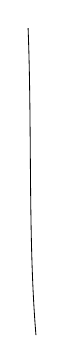
\begin{tikzpicture}[x=1mm,y=1mm]\draw[line width=.3pt] (1,0) .. controls (0,12) and (.5,26) .. (0,39);\end{tikzpicture}}}
\[
\det(\rho+\sigma)=\deleted{\underbrace{\det\rho}_{1}+\underbrace{\det\sigma}_{1}+\operatorname{Tr}(\sigma\rho)}
\]
% R343.05 | deletion | upper middle, lines 5--6 | et la relation équivaut
\deleted{and the relation is equivalent}
% R343.06 | display | middle, lines 6--9 | det sigma(1+sigma^{-1}rho)
\[
\begin{aligned}
\unsure{''}\quad
\det\unsure{(}\unsure{\deleted{\rho}\inserted{\sigma}}(1+\sigma^{-1}\rho)
&=\det\sigma\ \underbrace{\det(1+\sigma^{-1}\rho)}_{\underbrace{\det\sigma^{-1}\rho}_{(\det\sigma)^{-1}\det\rho}+\operatorname{Tr}(\underbrace{\sigma^{-1}\rho}_{-\sigma\rho})+1}\\
&=\overbrace{\det\sigma}^{1}+\overbrace{\det\rho}^{1}+\underbrace{\det\sigma}_{1}\operatorname{Tr}(\sigma^{-1}\rho)
\end{aligned}
\]
% R343.07 | margin note | diagonal left margin, beside lines 7--11 | calcul déjà fait
\margin{calculation already done See page \unsure{--} ? (cf. formula (69))}
% R343.08 | display | middle, line 10 | det(sigma+rho)=2+Tr(sigma^{-1}rho)
\[
\text{i.e.}\qquad\det(\sigma+\rho)=2+\operatorname{Tr}(\sigma^{-1}\rho)=2\unsure{-}\operatorname{Tr}\sigma\rho,\quad\text{thus}
\]
% R343.09 | text | middle, line 11 | la condition det N=0
the condition $\det N=0$ is equivalent to (69)
% R343.10 | display | middle, line 12 | Tr sigma rho=2
\[
\operatorname{Tr}\sigma\rho=2
\]
% R343.11 | text | lower, lines 13--17 | Pour prouver cette relation
To \deleted{\unsure{it}} prove this relation \inserted{(or \unsure{versions|neighboring ones} \unsure{tested|such})}, we can think of \deleted{starting}\inserted{proceeding} as earlier, \unsure{except that I} \unsure{have} started from (68) instead of (75). This is not entirely elucidated -- to return to the attack!
% R343.12 | text | bottom left | 342
\mspage{342}